%Part of/Parte di https://github.com/f-dinucci/appuntiMeccanicaFluidi/
%License/Licenza Creative Commons Attribution-ShareAlike 4.0 International (CC BY-SA 4.0) - attribution/attribuzione Francesco Di Nucci
%See also/Vedere anche https://creativecommons.org/licenses/by-sa/4.0/ and/e https://creativecommons.org/licenses/by-sa/4.0/legalcode
%
\section{Esperimento di Reynolds} 
\subsection{Esperimento di Reynolds}
Per lo studio dei flussi turbolenti è stato fatto l'esperimento di Reynolds: un tubo di vetro trasparente con del fluido e dell'inchiostro come tracciante.
Si vede grazie  al tracciante che ad un certo punto il moto diventa agitato.
 %
	\begin{figure}[ht]
		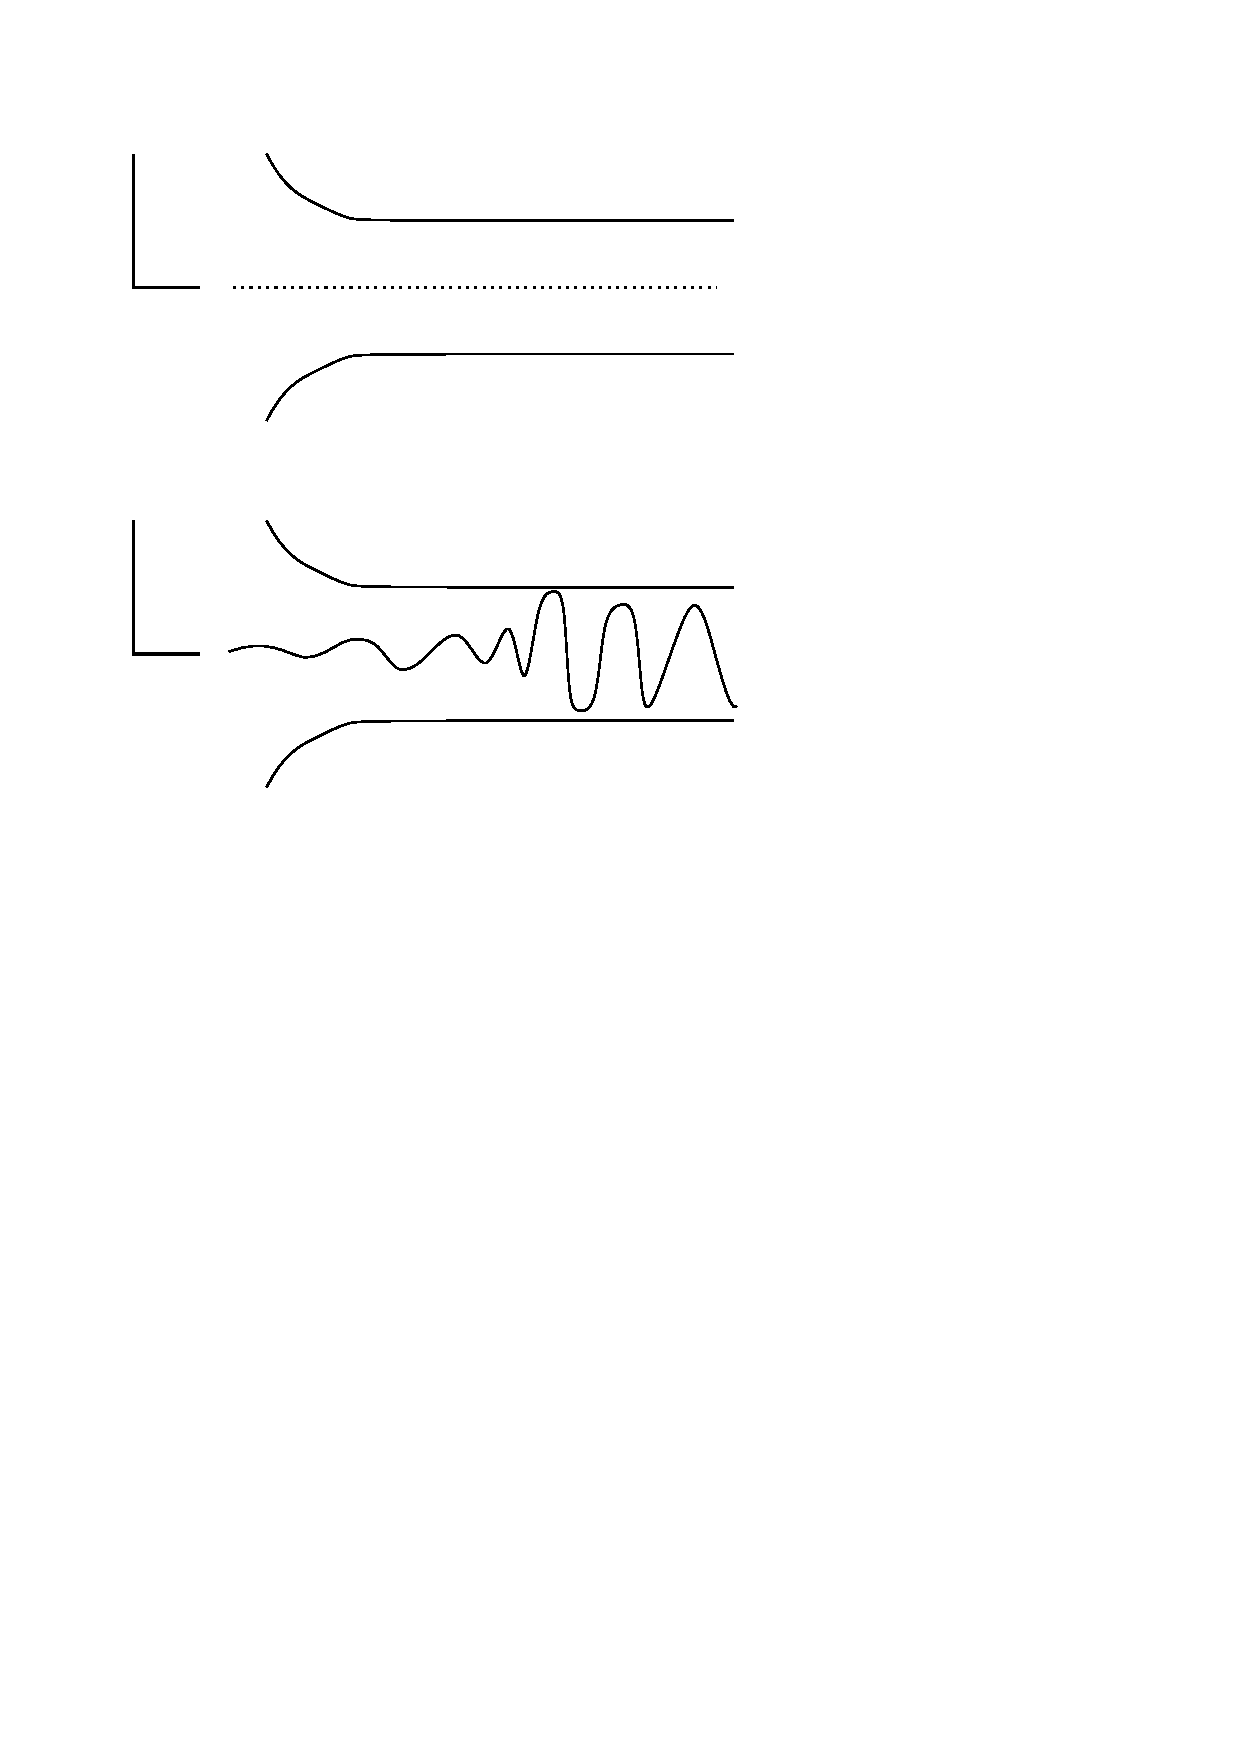
\includegraphics[scale=0.6]{./8.1 Esperimento di Reynolds/8.1-1}
		\centering
		\caption{Esperimento Reynolds}
	\end{figure}
%
Al variare del numero di Reynolds si possono avere differenti risultati con la stessa geometria.


\subsection*{Bibliografia 8.1}
\cite[Cap.\ 8.2]{CengelCimbala}\\
\cite[Cap.\ 12.1]{PnueliGutfinger}